% ========== Choix techniques ===========
\section{Choix techniques}

\subsection{Choix1}
    \begin{frame}
        \frametitle{Choix techniques}

		\begin{itemize}
		 \item Langage de programmation : \textbf{Java} \vspace{1cm}
		 \item Communication client-serveur : \textbf{RMI}
		 	\begin{itemize}
		 		\item Orienté objet
		 		\item Gestion des exceptions
		 	\end{itemize}
		\end{itemize}
    \end{frame}
    
\subsection{Choix2}
    \begin{frame}
    	\begin{itemize}
    		\item Interface graphique : \textbf{Slick2D} \vspace{3cm}
    		
    		\begin{picture}(3,9)
  			\put(50,-40){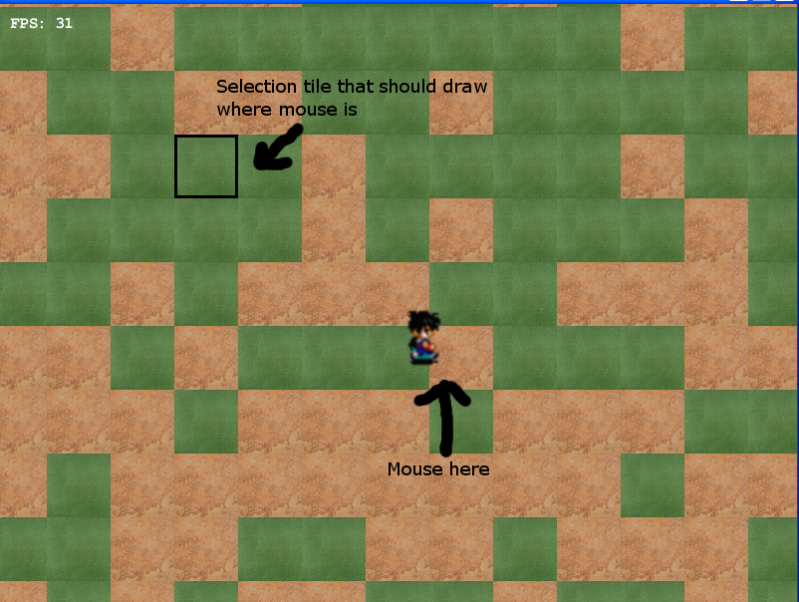
\includegraphics[scale=0.2]{ressources/illustration_slick2d.png}}
		\end{picture}
		\end{itemize}
		
		
	\end{frame}
